
\documentclass{article}
\usepackage{tikz}
\usepackage{tkz-euclide} % loads  TikZ and tkz-base
%\usetkzobj{all}
\usetikzlibrary{calc,math}

\begin{document}
\begin{figure}[!ht]
	\begin{center}
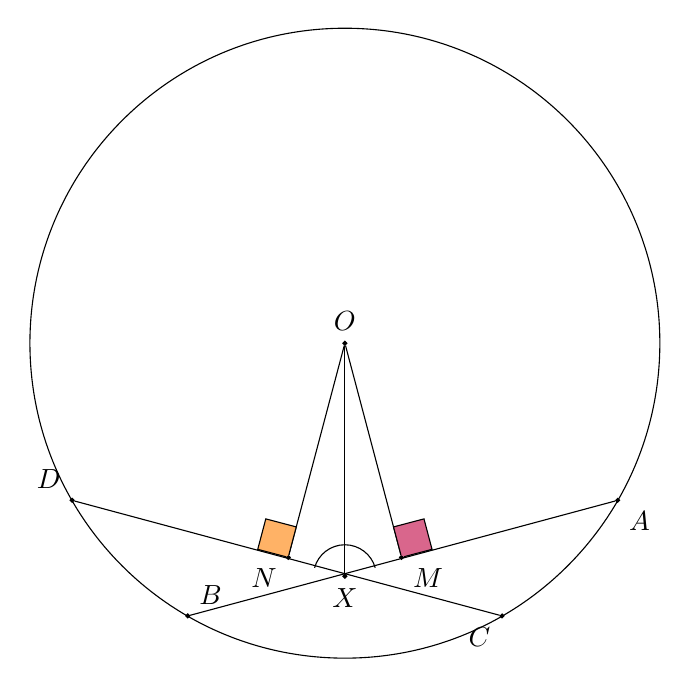
\begin{tikzpicture}
[scale=2,>=stealth,point/.style={draw,circle,fill = black,inner sep=0.5pt},]

%Triangle sides
\def\a{5}
\def\b{6}
\def\r{2}
%Coordinates of A
\def\pa{1.732}
\def\qa{0.998}
\def\pb{-1.732}
\def\qb{-0.998}
\def\mx{0.36}
\def\my{-1.36}
\draw (0,0) circle (2cm);
%Labeling points
\node (A) at (\pa,\qb)[point,label=below right:$A$] {};
\node (B) at (\qb, \pb)[point,label=above right:$B$] {};
\node (M) at (0.36,-1.36)[point,label=below right:$M$] {};
\node (N) at (-0.36,-1.36)[point,label=below left:$N$] {};
\node (X) at (0,-1.48)[point,label=below:$X$] {};

\node (C) at (\qa,\pb)[point,label=below left:$C$] {};
\node (D) at (\pb, \qb)[point,label=above left:$D$] {};
%\node (Y) at (\q, 0)[point,label=left:$Y$] {};

\node (O) at (0,0)[point,label=above:$O$]{};

%Drawing triangle ABC
\draw (A) --  (B);
\draw (X)-- (O);
\draw (C) --  (D);
\draw (N)-- (O);
\draw (M)-- (O);
%Drawing medians BE and CF
%\draw (D) -- (E);
%\draw (D) -- (F);
%\draw (O) -- (B);
%\draw (O) -- (C);
%Drawing EF
%\draw (E) -- (F);

%Labeling sides
%\node [right] at ($(A)!0.5!(E)$) {$\frac{b}{2}$};
%\node [right] at ($(C)!0.5!(E)$) {$\frac{b}{2}$};
%\node [left] at ($(B)!0.5!(F)$) {$\frac{c}{2}$};
%\node [left] at ($(A)!0.5!(F)$) {$\frac{c}{2}$};

%Angles
\tkzMarkRightAngle[fill=purple!60,size=.2](A,M,O)
\tkzMarkRightAngle[fill=orange!60,size=.2](O,N,D)
%\tkzMarkAngle[fill=green!60,size=.3](O,B,A)
%
\tkzMarkAngle[fill=red!60,size=.2](O,X,D)
\tkzMarkAngle[fill=green!60,size=.2](A,X,O)
%%
%\tkzMarkAngle[fill=yellow!60,size=.2](A,D,E)
%\tkzMarkAngle[fill=yellow!60,size=.2](A,O,B)
%%
%\tkzMarkAngle[fill=orange!60,size=.2](F,D,A)
%\tkzMarkAngle[fill=orange!60,size=.2](C,O,A)
%
%\tkzMarkAngle[fill=blue!60,size=.3](E,A,F)
\end{tikzpicture}
	\end{center}
\caption{If two equal chords of a circle intersect within the circle, the line joining the point of intersection to the center makes equal angles with the chords}
\label{fig:step2}	
\end{figure}
\end{document}
